\documentclass[a4paper,11pt]{report}
%
%--------------------   start of the 'preamble'
%
\usepackage{graphicx,amssymb,amstext,amsmath}
%
%%    homebrew commands -- to save typing
\newcommand\etc{\textsl{etc}}
\newcommand\eg{\textsl{eg.}\ }
\newcommand\etal{\textsl{et al.}}
\newcommand\Quote[1]{\lq\textsl{#1}\rq}
\newcommand\fr[2]{{\textstyle\frac{#1}{#2}}}
\newcommand\miktex{\textsl{MikTeX}}
\newcommand\comp{\textsl{The Companion}}
\newcommand\nss{\textsl{Not so Short}}
%
%---------------------   end of the 'preamble'
%
\begin{document}
%-----------------------------------------------------------
\title{Report of MSR Data Mining Challenge 2012}
\author{Laura Bledaite \& Martynas Pumputis}
\maketitle
%-----------------------------------------------------------
\begin{abstract}\centering
A couple of sentences on three or four lines to summarise your work.\\ 
This is a \LaTeX\ template for undergraduate project reports.\\
Its detailed contents evolve to reflect FAQs.
\end{abstract}
%-----------------------------------------------------------
\tableofcontents
%-----------------------------------------------------------
\chapter{Introduction}
\chapter{Simple Statistics}
First of all, we tried to make some statistics about the data in order to see how it looks and get some ideas about what might be done and/or draw some conclusions.
The first thing we looked at was the comment frequencies in a bug. We have 14975 comments related to some bug in total. The maximum number of comments related to one bug was 25, the minimum - 1, the average - 4.5228714524207. The graph showing the distribution of the comment frequencies in a bug is shown in Figure~\ref{fig:com_freq}. This lets us conclude that most of the bugs do not have many comments, most often they have only one or a couple of them. Actually, 79\% of the bugs have $<=5$ comments.

\begin{figure}[ht!]
\centering
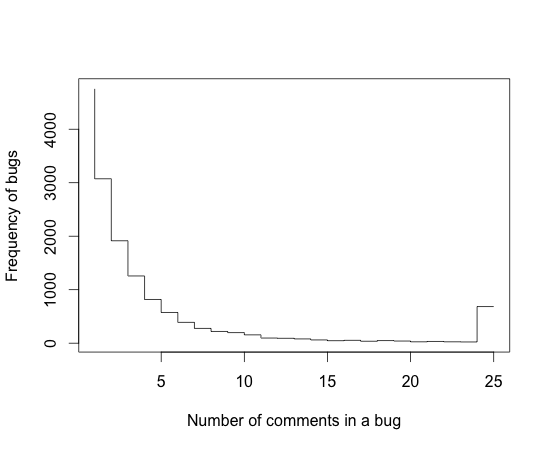
\includegraphics[width=.7\textwidth]{comment_frequencies.png}
\caption{Comment frequencies in a bug.}
\label{fig:com_freq}
\end{figure}

Secondly, we were interested in how long it takes to solve a bug. In order to find it, we filtered the data taking only the bugs that are already closed and calculates the times from opening untill closing in days. There were 6345 closed bugs. The minimum time required to solve the bug took 0.0001967591 days, maximum - 1365.347, average - 72.44017. Figure~\ref{fig:res_times} shows the distribution of the time required for resolving a bug.

\begin{figure}[ht!]
\centering
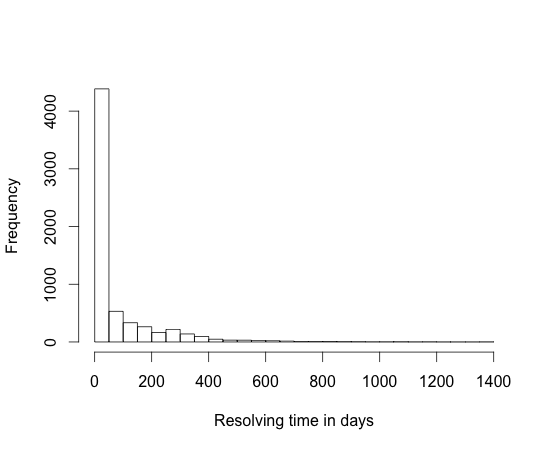
\includegraphics[width=.7\textwidth]{resolving_times.png}
\caption{Histogram of bug resolving times.}
\label{fig:res_times}
\end{figure}
 
\begin{figure}[ht!]
\centering
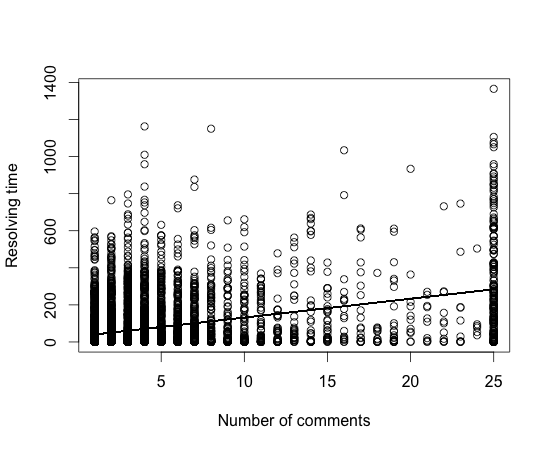
\includegraphics[width=.7\textwidth]{comments_time.png}
\caption{Bug resolving time realtionship with the number of comments in a bug.}
\label{fig:com_time}
\end{figure}

Moving more in detail, we made an assumption that maybe the resolving time and the number of comments are related, i.e. maybe there exists a tendency that more comments mean faster resolving of a bug. Figure~\ref{fig:com_time} shows the relationship between the number of comments in a bug and the time required to resolve a bug. A line in Figure~\ref{fig:com_time} shows an attempt to adjust the linear regression model for the data using the number of comments as a predictor variable. The predicted model looks like this:
\[
ResolvingTime=30.0465 + 10.1493 \cdot NumberOfComments.\]
The results of the general linear model are shown in Table~\ref{tbl:glm}.

\begin{table}[ht!]
\centering
\begin{tabular}{|c|c|c|c|c|c|c|}
\hline
Coefficients & Estimate Std. & Error & t value & {$Pr(>|t|)$}\tabularnewline
\hline
\hline
(Intercept) & 30.0465 & 2.0509 & 14.65 & {$<2e-16 $}***\tabularnewline
\hline
NumberOfComments & 10.1493 & 0.3108 & 32.66 & {$<2e-16$}***\tabularnewline
\hline
\end{tabular}
\footnotemark{Signif. codes:  *** 0.001 ** 0.01 * 0.05}
\caption{Linear regression results.}
\label{tbl:glm}
\end{table}

Inspite of the fact, that the results of the general linear model prove the coefficient of the number of comments not be be equal 0, the data do not seem to be very well explained by the model adjusted. This might have happened because it may happen naturally, that the longer the bug is being solved, the more comments it gets, but it does not give any more information. Contrarily, we expect that the more comments a bug gets, the faster it is resolved. To address this issue, we decided to take a look at the comments' density in a time period and its relationship to the resolving time. And actually results show that there exist such a relationship. Figure~\ref{fig:density_time} does not suggest the fitting model for the data, but it shows several data properties. Firstly, it is easy to notice that whenever a bug is very dense in comments, it will most likely be resolved very fast. On the other hand, it does not mean that a bug which is sparse in comments cannot be resolved fast. Bugs having few comments have similar probability to be solved fast or slow.

\begin{figure}[ht!]
\centering
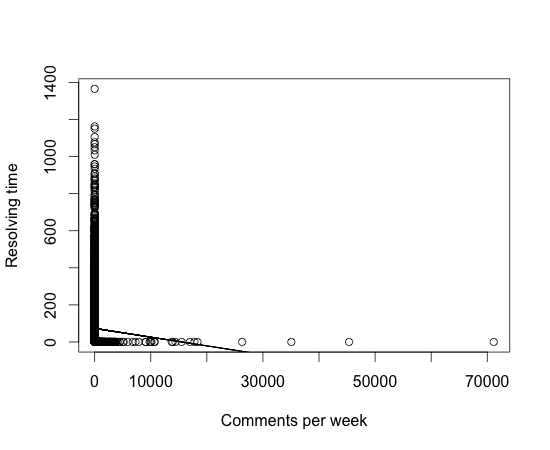
\includegraphics[width=.7\textwidth]{density_time.png}
\caption{Bug resolving time realtionship with the comment density in a bug.}
\label{fig:density_time}
\end{figure}


%-----------------------------------------------------------
\addcontentsline{toc}{chapter}{\numberline{}Bibliography}

\begin{thebibliography}{9999}%\enlargethispage{\baselineskip}
\bibitem[AC]{AC}A~Cottrell, \textsl{Word Processors: Stupid and
Inefficient},
\\ \mbox{}\hfill\texttt{www.ecn.wfu.edu/\~{}cottrell/wp.html}
\bibitem[BR]{BR}Visit \texttt{www.dur.ac.uk/library/using/guides/}
and click on \Quote{Writing your bibliography and citing references}.
\bibitem[ESL]{ESL}L~Truss, \textsl{Eats, Shoots and Leaves}, Profile
  Books 2003\\ \mbox{}\hfill(ISBN~\texttt{1-86197-612-7}).
\bibitem[GRM]{GRM}M~Goossens, S~Rahtz and F~Mittelbach,\\
  \mbox{}\hfill \textsl{The \LaTeX\ Graphics Companion},
  Addison-Wesley, 1997\\  \mbox{}\hfill(ISBN~\texttt{0-201-85469-4}).
\bibitem[IM]{IM} \textsl{ImageMagick}, {\tt%
www.dur.ac.uk/its/software/application/\dots
\\ \mbox{}\hfill\dots?application=ImageMagick}
\bibitem[LAT]{LAT} \textsl{\LaTeX\ stuff},
	\texttt{maths.dur.ac.uk/Ug/projects/resources/latex/}
\bibitem[MEM]{MEM} \textsl{Memoir document class},\\ \mbox{}\hfill
   \texttt{www.ctan.org/tex-archive/macros/latex/contrib/memoir/}
\bibitem[MG]{MG}F~Mittelbach and M~Goossens \etal, \textsl{The
\LaTeX\ Companion},\\  \mbox{}\hfill Addison-Wesley, 2nd ed. 2004
(ISBN~\texttt{0-201-36229-6}).
\bibitem[MKT]{MKT} \textsl{MikTex Project Page}, \texttt{www.miktex.org}
\bibitem[NSS]{NSS}T~Oetiker, H~Partl, I~Hyna and E~Schlegl,\\
\mbox{}\hfill
\textsl{The Not So Short Introduction to \LaTeXe},\\ \mbox{}\hfill{\tt
www.ctan.org/tex-archive/info/short}
\bibitem[PS]{PS} \textsl{Photoshop}, {\tt%
www.dur.ac.uk/its/software/application/\dots
\\ \mbox{}\hfill\dots?application=Adobe+Photoshop}
\bibitem[TXC]{TXC} \textsl{TeXnicCenter}, \texttt{www.toolscenter.org}
\bibitem[WDT]{WDT} \textsl{WinEdt}, \texttt{www.winedt.com}
\bibitem[WL]{WL} \textsl{Wikibook on \LaTeX}, \texttt{%
	en.wikibooks.org/wiki/Latex}
\bibitem[WO]{WO} \textsl{Controlling widows and orphans}, 
\\ \mbox{}\hfill\texttt{www.tex.ac.uk/cgi-bin/texfaq2html?label=widows}
\bibitem[WSH]{WSH} \textsl{WinShell}, \texttt{www.winshell.de}
\end{thebibliography}
\vfill
\begin{flushright}\small Prepared in \LaTeXe\ by RCJ\end{flushright}

%-----------------------------------------------------------
\appendix
\include{app4}
\include{app1}
\include{app2}
\include{app5}
\include{app3}
%-----------------------------------------------------------
\end{document}
